
\chapter{Evaluation of SHAMPU}
In order to assess the capabilities of SHAMPU, we plan and run experiments designed to evaluate the SHAMPU framework according to the following use-cases:
\begin{itemize}
	\item{\textbf{Scheduled data-transmission}} \hfill \\ In order for SHAMPU to work as a debugging and logging platform, the base station needs to periodically receive data from all the nodes in the network. Furthermore the base station has to be able to send commands to nodes in the network.
	\item{\textbf{Unscheduled data-transmission}} \hfill \\ There are several cases, where it is not feasible to use a scheduled data-transmission. Because either the data only needs to be transmitted once, or it is not know at what point in time the transmission happens: 
	\begin{itemize}
		\item{}Reprogramming of a node: SHAMPU is able to reprogram the attached node. For this process, SHAMPU needs to receive a new firmware, which can amount to several hundred kB.
		\item{}SHAMPU RAM-Dumps: SHAMPU has 128kB of RAM, which can be used to save collected data during an experiment. At the end of the experiment the complete memory needs to be transmitted back to the base station.
	\end{itemize}
\end{itemize}
	
To evaluate ANT according to these two use-cases, we identified three metrics which indicate how well a use-case can be handled:
	\begin{itemize}
		\item {\textbf{Data throughput }} \hfill \\ The speed with which ANT can transmit data directly affects the network performance and how many nodes can be part of the network at once. ANT provides three different data types which can be used to transport data: Broadcast data and acknowledge data can be used for scheduled data-transmission. Burst mode can be used for unscheduled data-transmission. 		
		
		\item {\textbf{Message delay}} \hfill \\ A SHAMPU base station not only acts as a data sink for incoming logging information, but is also able to send commands to other SHAMPU devices in the network.
		It is thus important to know how long it takes ANT to verify whether a message was correctly received or not.
		
		\item {\textbf{Communication range}} \hfill \\ Since SHAMPU is architecture independent it can be used in different situations. Therefore it is important to know, how far away from the base station the nodes can be placed. As SHAMPU focuses on energy efficiency, it might also be viable to reduce the range for smaller set ups to save even more energy.
	\end{itemize}

To cover the mentioned metrics we designed different experiments, which test one or more of the described categories. The following section describes the experiments according to the following template:

\begin{description}
	\item{\textbf{Description}} \hfill \\ A description of the experiment and the category being evaluated.
	\item{\textbf{Use-Case}} \hfill \\ The use-case which the experiment tries to test.
	\item{\textbf{Network topology and pseudo code}} \hfill \\ A diagram of the network topology in which the experiment is run and pseudo code which describes the program being run on the master and the slave. Missing values are default values and described in section \ref{sec:commonPara}.
	\item{\textbf{Testing methodology}} \hfill \\ A description how the experiment is performed.
	\item{\textbf{Result}} \hfill \\ The results of the experiment and any additional data collected during the experiment.
\end{description}

\newpage

\section{Common experiment parameters}
\label{sec:commonPara}
\begin{figure}[H]
	\centering
	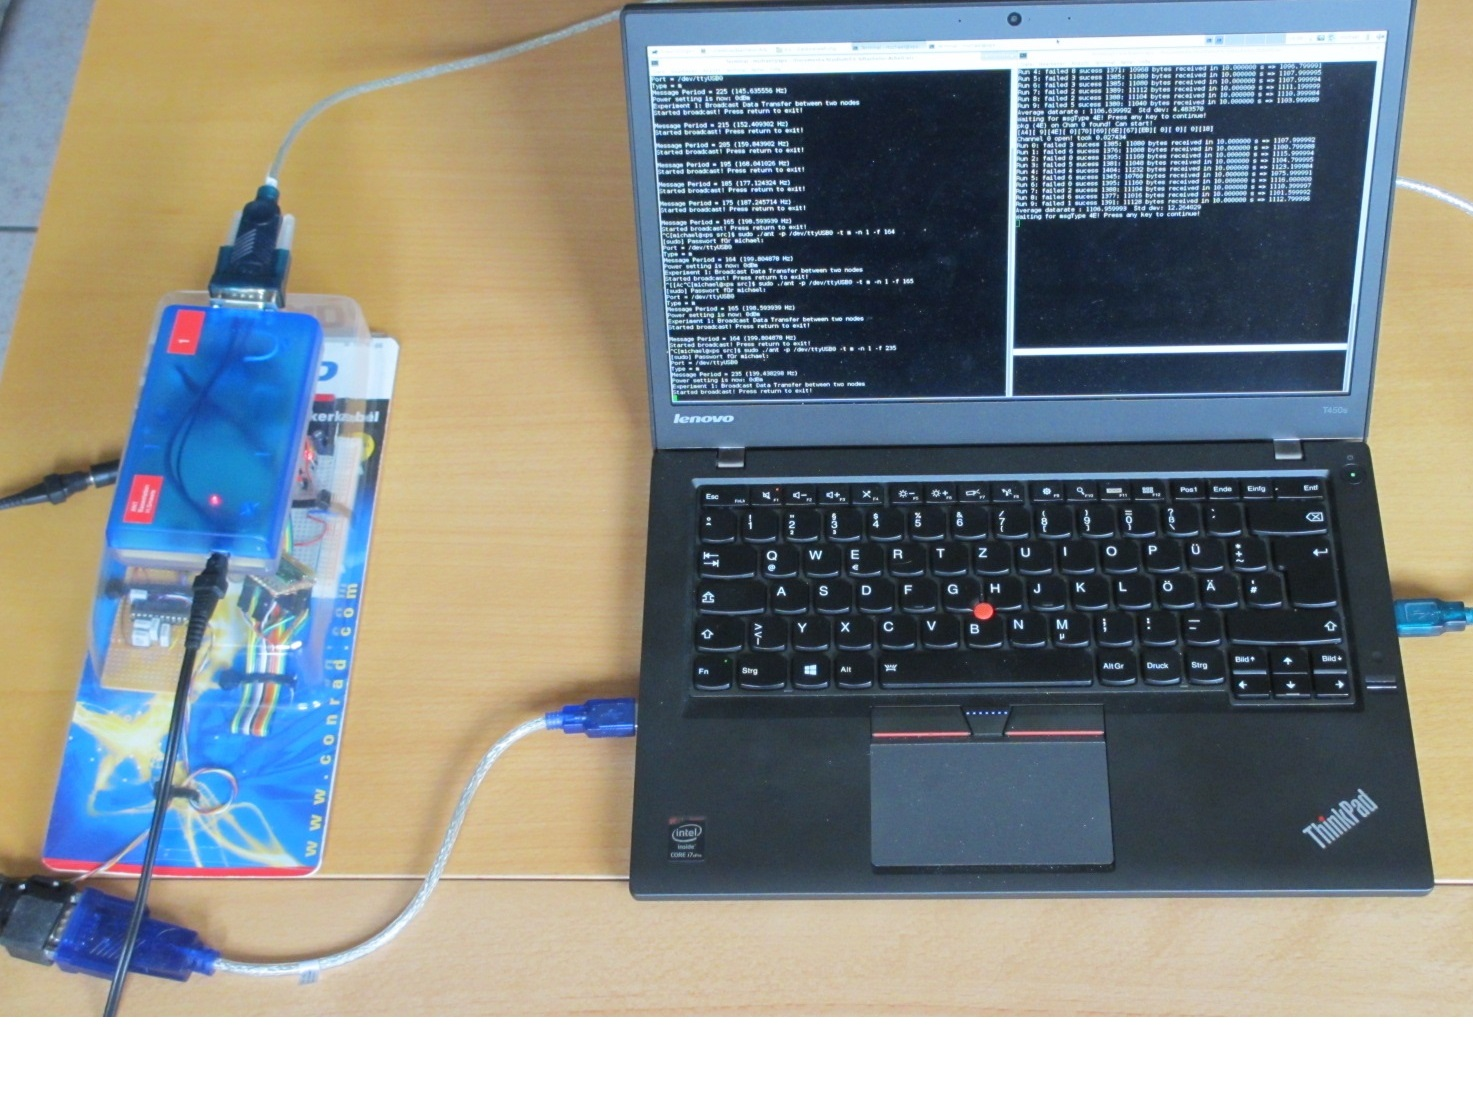
\includegraphics[scale=.75]{content/images/expSetup.JPG}
	\caption{Experiment set up}\label{fig:expSetup}
\end{figure}

If not otherwise noted in the description each experiment was run in the Mobility Lab of the Networked Embedded Systems group at the University of Duisburg-Essen (SA 327), with the two base stations in the configuration which can be seen in figure \ref{fig:expSetup}. The following table describes the parameters which were used in the experiments.

\begin{table}[H]
	\centering
	\begin{tabular}{|l|c|c|}
		\hline
		Device number        & 33    & \multirow{3}{*}{\begin{tabular}[c]{@{}c@{}}Channel ID\\ (see section \ref{sec:ANTchan})\end{tabular}}   \\ \cline{1-2}
		Device type          & 1     &                                                                                                         \\ \cline{1-2}
		Transmission type    & 1     &                                                                                                         \\ \hline
		ID\_CHAN1            & 0     & \multirow{2}{*}{\begin{tabular}[c]{@{}c@{}}Configuration\\ for the first channel\end{tabular}}          \\ \cline{1-2}
		FREQ\_CHAN1          & 66 Hz &                                                                                                         \\ \hline
		ID\_CHAN2            & 1     & \multirow{2}{*}{\begin{tabular}[c]{@{}c@{}}Configuration\\ for the second channel\end{tabular}}         \\ \cline{1-2}
		FREQ\_CHAN2          & 77 Hz &                                                                                                         \\ \hline
		STD\_FREQ            & 8192  & 4 Hz (default frequency)                                                                                \\ \hline
		min\_Channel\_Period & 164   & 199.8 Hz (closest to 200 Hz)                                                                            \\ \hline
		max\_Channel\_Period & 65535 & 0.5 Hz (smallest frequency)                                                                             \\ \hline
		STD\_POWER           & 0 dBm & 1 mW (default transmit power)                                                                           \\ \hline
	\end{tabular}
	\caption{ANT default configuration}
\end{table}

There is an important difference between the message period used in the pseudo code and the frequency used in the figures which display the results. The period describes the size of the gap between two messages, the frequency describes how many messages are sent in 1 second. The channel period $p$ can be used to calculate the frequency of the messages $f_t = \frac{32678s^{-1}}{p}$. For example a message period of 8192 results in a message frequency of 4 Hz, which means that 4 messages are send every second.

ANT supports different transmit power levels: 0 dBm, -5 dBm, -10 dBm and -20 dBm. dBm is a way to express broadcast power as a power ratio in decibels. The power of the broadcast $p$ can be calulated as follows $p = 1mW * 10^{\frac{x}{10}}$.

Furthermore in experiments which measure data throughput, we show maximum theoretical value for each frequency. This is the maximum value which can be achieved, if there are no transmission errors and no interference with other channels. The value depends on the message frequency $f$ and be calculated as follows: $rate_{max}(f) = 8*f$. Each message contains contains a payload of 8 bytes and we send $f$ messages each second.
\newpage

\section{Experiment 1: Broadcast Data Transfer between two nodes}
\begin{description} 
	\item{\textbf{Description}} \hfill \\ Broadcasting is one way of periodically transmitting data between two or more ANT nodes. Since all broadcast packets are synchronized to a fixed time-slot, the data throughput can be increased by decreasing the channel period. The experiment itself is split into two parts. In the first part we try to determine the highest possible data throughput. Also we try to determine whether the channel period has an effect on the time it takes for a slave node to find and join an existing channel. The second part is a test of the highest detected data throughput. Here we try to evaluate if there are any variations of the data throughput over a much longer interval.	
	\item{\textbf{Use-Case}} \hfill \\ Scheduled data-transmission	
	\item{\textbf{Network topology and pseudo code}} \hfill \\ 
	\begin{figure}[H]
		\centering
		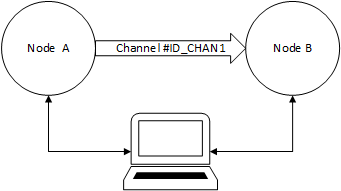
\includegraphics[scale=1]{content/images/exp_topo.png}
		\caption{Topology experiment 1}
	\end{figure}
	\begin{code}[H]
		\begin{verbatim}
		channelPeriod = max_Channel_Period
		while (channelPeriod >= min_Channel_Period)
		  ANT_SetChannelPeriod(ID_CHAN1, channelPeriod)
		  ANT_OpenChannel(ID_CHAN1, ANT_Bidirectional_Master)
		  ANT_SendBroadcastData(ID_CHAN1, [0x01, 0x02, 0x03, 0x04])
		  wait_for_user_input()
		  ANT_CloseChannel(ID_CHAN1)
		  if (channelPeriod >= 0x00FF)
		    channelPeriod = channelPeriod >> 1
		  else
		    channelPeriod = channelPeriod - 10
		\end{verbatim}
		\caption{Broadcast data single channel (Master)}\label{lst:mExp1}
	\end{code}
	
	\begin{code}[H]
		\begin{verbatim}
		channelPeriod = max_Channel_Period
		while (channelPeriod >= min_Channel_Period) 
		  for (i in 0..10) 
		    ANT_SetChannelPeriod(ID_CHAN1, channelPeriod)
		    ANT_OpenChannel(ID_CHAN1, ANT_Bidirectional_Slave)
		    count = 0
		    for (100 seconds) 
		      if (receivedPacket() == ANT_BROADCAST_DATA)
		        count++;			  
		    print (count * 8 / 100) + " Bytes per second"
		    wait_for_user_input()
		    ANT_CloseChannel(ID_CHAN1)
		  if (channelPeriod >= 0x00FF)
		    channelPeriod = channelPeriod >> 1
		  else
		    channelPeriod = channelPeriod - 10
		\end{verbatim}
		\caption{Broadcast data single channel (Slave)}\label{lst:sExp1}
	\end{code}	
	\item{\textbf{Testing methodology}} \hfill \\Experiment 1 is split into two parts.
	In the first part node A acts as the master and node B as the slave. For both nodes the channel period is set to the highest value and the channel is opened. Node B records how long it takes to join the channel and how many bytes it receives over a 100s interval. The measurement is repeated 10 times and the average values are saved. Then the channel period is decreased and the process is repeated.\\ 
	In the second part of the experiment, the channel period is set to the value which achieved the highest speed. The experiment is then left running for a period of 10 hours and the data throughput is recorded in one continuous run.
	\item{\textbf{Result}} \hfill \\  
	\begin{figure}[H]
		\centering
		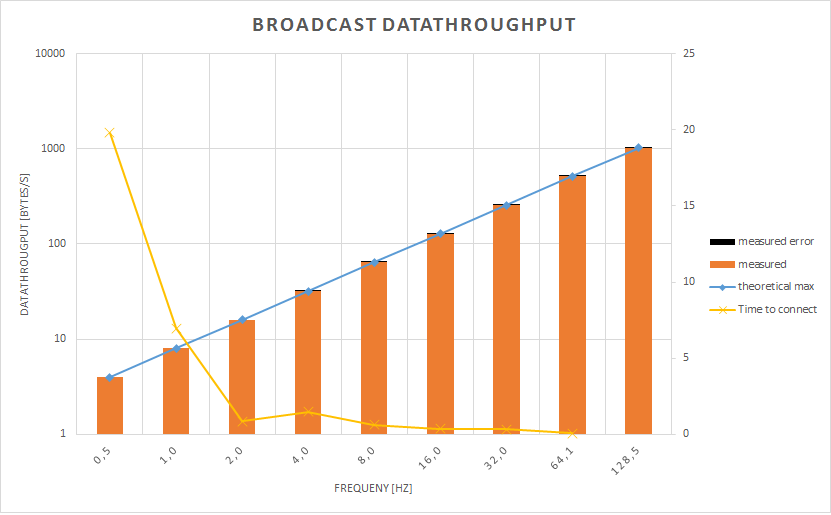
\includegraphics[scale=0.5]{content/images/exp1_norm.png}
		\caption{Broadcast data rate (0.5Hz - 198.6Hz)}\label{fig:exp1norm}
	\end{figure}
	
	Figure \ref{fig:exp1norm} shows the transmission speeds achieved for the different frequencies. Up to a frequency of 128 Hz, the measured data rate matches the expected theoretical maximum rate. For the highest measured frequency (198.6 Hz), the data rate is much lower than the maximum rate. The measured errors are insignificant. Therefore the frequencies between 128 Hz and 198.6 Hz were analyzed in more detail. 
		
	The time it takes for a Node to join a channel falls rapidly once the frequency is above 1 Hz. For frequencies above 64 Hz, the time it takes to join a channel becomes negligible, with times around 75 ms (see Figure \ref{fig:exp1norm}). All the measured values are below the specified worst case channel acquisition times of the ANT protocol \cite{AntChan}.
	
	\begin{figure}[H]
		\centering
		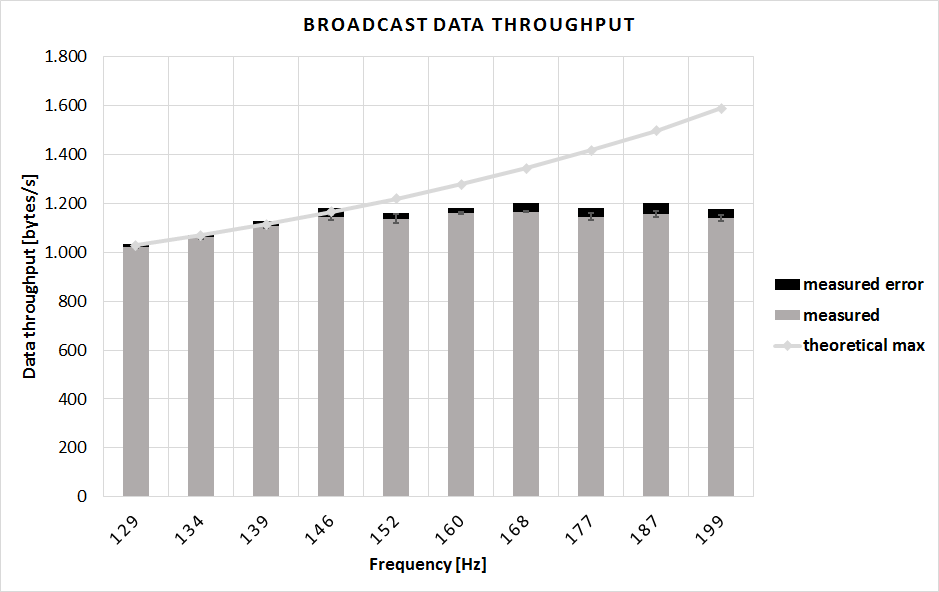
\includegraphics[scale=0.5]{content/images/exp1_detail.png}
		\caption{Broadcast data rate (129Hz - 198.6Hz)}\label{fig:exp1between}
	\end{figure}
	As seen in figure \ref{fig:exp1between} the measured data rates for frequencies above 140 Hz all fall short of the expected values. The average data throughput of these frequencies remains consistently at around 1100 Bps. The experiment was repeated multiple times, running it at different times and places, thus an environmental factor can be excluded. That means, the reason for the upper limit has to be found with the test set up itself. See section \ref{sec:dataThrougput} for a discussion about possible reasons for this upper limit.
	
	\begin{figure}[H]
		\centering
		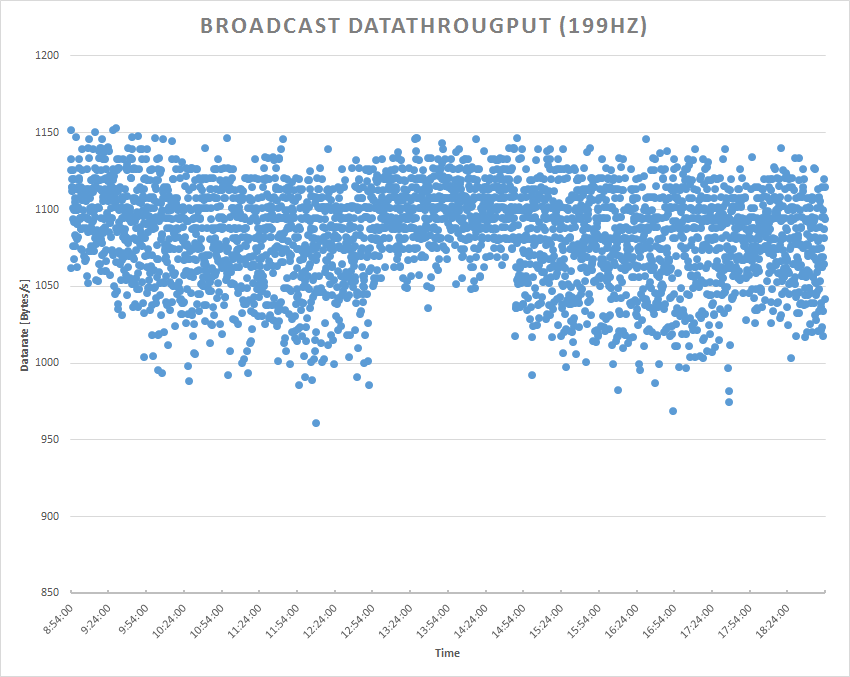
\includegraphics[scale=0.5]{content/images/exp1_long.png}
		\caption{Broadcast data rate over time (198.6Hz)}\label{fig:exp1long}
	\end{figure}
	Figure \ref{fig:exp1long} shows the transmission speed for the highest supported frequency 198.6 Hz over time. The results show that the data throughput stays fairly consistent at around 1100 Bps with a standard deviation of only 30 Bps, or 2.7\%. Interesting to note is the time period from 1:00PM to 2:50 PM, where the deviation from the average is much smaller. The exact reason for this phenomenon in unknown, since during this time period the environment of the test set up did not change in any known way.
\end{description}
\newpage

\section{Experiment 2: Broadcast Data Transfer with two channels}
\begin{description} 
	\item{\textbf{Description}} \hfill \\ In experiment 1 we determined the channel period, which allows for the maximum throughput. In this experiment we try to determine, how the maximum throughput is affected by the amount of channels in the network. SHAMPU needs two channels, so it can work correctly: One channel which sends data from the base station to the nodes in order to control them and another channel by which the nodes can send debugging and other information.
	\item{\textbf{Use-Case}} \hfill \\ Scheduled data-transmission	
	\item{\textbf{Network topology and pseudo code}} \hfill
	\begin{figure}[H]
		\centering
		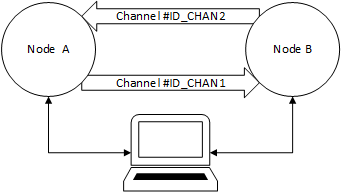
\includegraphics[scale=1]{content/images/exp2_topo.png}
		\caption{Topology experiment 2}
	\end{figure}
	\begin{code}[H]
		\begin{verbatim}
		channelPeriod = max_Channel_Period
		while (channelPeriod >= min_Channel_Period) 
		  ANT_SetChannelPeriod(ID_CHAN1, channelPeriod)
		  openChannel(ID_CHAN1, ANT_Bidirectional_Master)
		  ANT_SendBroadcastData(ID_CHAN1, [0x01, 0x02, 0x03, 0x04])
		  ANT_SetChannelPeriod(ID_CHAN2, channelPeriod)
		  openChannel(ID_CHAN2, ANT_Bidirectional_Slave)
		  count = 0
		  for (100 seconds) 
		    if (receivedPacket() == ANT_BROADCAST_DATA)
		      count++			
		  print (count * 8 / 10) + " Bytes per second"
		  wait_for_user_input()
		  ANT_CloseChannel(ID_CHAN1)
		  ANT_CloseChannel(ID_CHAN2)
		  if (channelPeriod >= 0x01FF)
		    channelPeriod = channelPeriod >> 1
		  else
		    channelPeriod = channelPeriod - 10
		 \end{verbatim}
		\caption{Broadcast data transfer two channels (Master)}\label{lst:mExp2}
	\end{code}
	
	\begin{code}[H]
		\begin{verbatim}
		channelPeriod = max_Channel_Period
		while (channelPeriod >= min_Channel_Period)
		  ANT_SetChannelPeriod(ID_CHAN1, channelPeriod)
		  openChannel(ID_CHAN1, ANT_Bidirectional_Slave)
		  ANT_SetChannelPeriod(ID_CHAN2, channelPeriod)
		  openChannel(ID_CHAN2, ANT_Bidirectional_Master)
		  ANT_SendBroadcastData(ID_CHAN2, [0x01, 0x02, 0x03, 0x04])
		  count = 0
		  for (100 seconds) 
		    if (receivedPacket() == ANT_BROADCAST_DATA)
		      count++			
		  print (count * 8 / 10) + " Bytes per second"
		  wait_for_user_input()
		  ANT_CloseChannel(ID_CHAN1)
		  ANT_CloseChannel(ID_CHAN2)
		  if (channelPeriod >= 0x01FF)
		    channelPeriod = channelPeriod >> 1
		  else
		    channelPeriod = channelPeriod - 10
		\end{verbatim}
		\caption{Broadcast data transfer two channels (Slave)}\label{lst:mExp2}
	\end{code}
	
	\item{\textbf{Network topology and pseudo code}} \hfill \\ The two nodes are placed right next to each other.
	
	\item{\textbf{Testing methodology}} \hfill \\ In this experiment each node acts as a master for a different channel. Node A is the master for Channel 0 and Node B is the master for Channel 1. The measurements themselves are identical to the ones in experiment 1, except that the data is recorded on both nodes. The channel period is then decreased until the data throughput no longer increases, or the connections breaks completely.
	
	\item{\textbf{Result}} \hfill \\  	
	\begin{figure}[H]
		\centering
		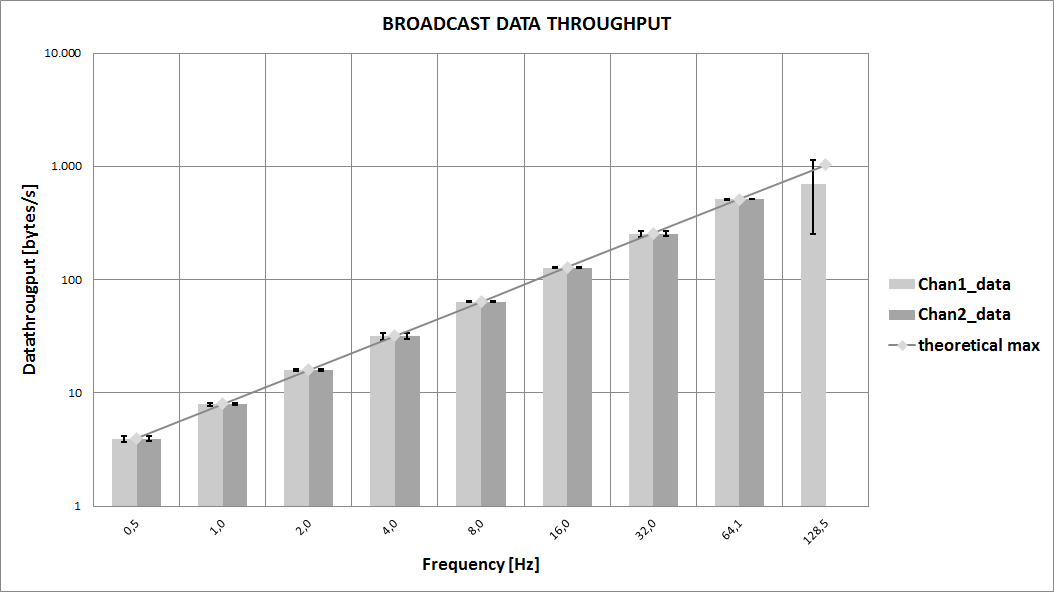
\includegraphics[scale=0.5]{content/images/exp2_norm.png}
		\caption{Broadcast data through - 2 channels (0.5Hz - 129Hz)}\label{fig:exp2low}
	\end{figure}
	Figures \ref{fig:exp2low} shows the results of the measurements, the left bar displaying the throughput for channel 1, the right bar displaying the throughput for channel 2. Just as in experiment 1 the  line shows the theoretical maximum of the data throughput for the given frequency. Up to a frequency of 64 Hz the data throughput increases with the frequency for both channels and matches the maximum value very closely. However the data throughput of channel 2  drops to zero at 128 Hz, while the data throughput of channel 1 almost matches the expected value, although the standard deviation indicates performance problems in this channel as well.
		\begin{figure}[H]
			\centering
			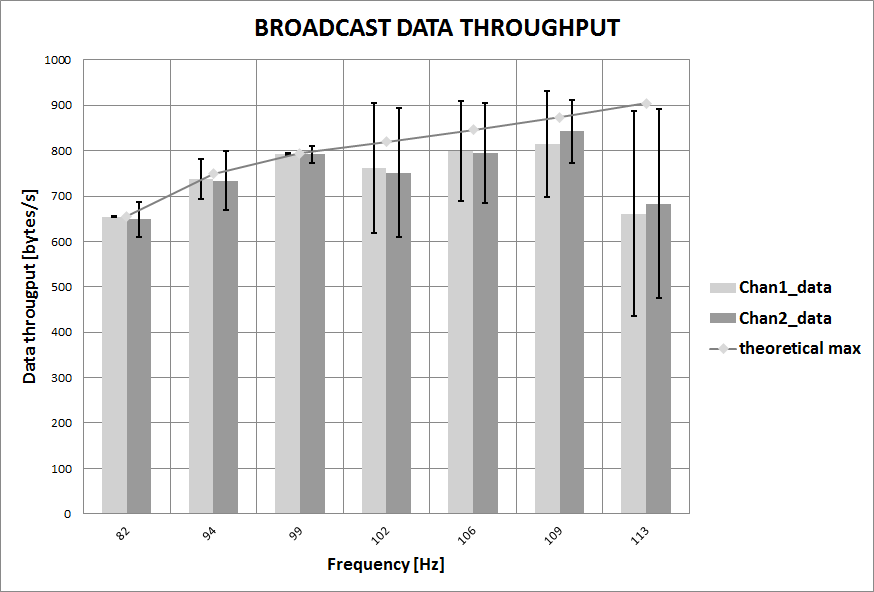
\includegraphics[scale=0.5]{content/images/exp2_detail.png}
			\caption{Broadcast data through - 2 channels (64Hz - 129Hz)}\label{fig:exp2high}
		\end{figure}
	To further investigate this drop off, figure \ref{fig:exp2high} shows the data throughput for chosen frequencies between 82 Hz and 113 Hz. Up to a frequency of 99 Hz the data throughput matches the expected values. For frequencies over 100 Hz however the data throughput drops off, while the measured errors increase. From this result we conclude two things: The 200 Hz capacity of the ANT chip is split between all channels the chip in part of. In this case each chip can broadcast with 100 Hz and receive with 100 Hz, resulting in a data throughput of around 800 Bps for each channel. Above 100 Hz the increased standard deviation can be interpreted as an indication of interferance between the sending and receiving unit of the ANT chip. This interference eventually leads to a breakdown of the data throughput at even higher frequencies.	
	See section \ref{sec:dataThrougput} for a discussion about this upper limit. 	
	
\end{description}
\newpage


\section{Experiment 3: Acknowledge Data Transfer between two nodes}
\begin{description} 
	\item{\textbf{Description}} \hfill \\ This experiment is almost identical with experiment 1. The main difference is that we use acknowledge data instead of broadcast. It is also important to note that the master records how many successful packets are transmitted. The main goal of the experiment is to see whether the data throughput is decreased compared to broadcast data, especially for smaller channel periods.
	\item{\textbf{Use-Case}} \hfill \\ Scheduled data-transmission
	\item{\textbf{Network topology and pseudo code}} \hfill \\
	\begin{figure}[H]
		\centering
		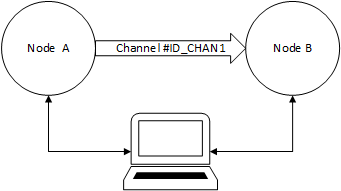
\includegraphics[scale=1]{content/images/exp_topo.png}
		\caption{Topology experiment 3}
	\end{figure}
	\begin{code}[H]
		\begin{verbatim}
		channelPeriod = max_Channel_Period
		while (channelPeriod >= min_Channel_Period) 
		  ANT_SetChannelPeriod(ID_CHAN1, channelPeriod)
		  ANT_OpenChannel(ID_CHAN1, ANT_Bidirectional_Master)
		  count = 0
		  for (10 seconds) 
		    ANT_SendAcknowledgedData(ID_CHAN1, [0x01, 0x02, 0x03, 0x04])	   
		    wait_for_ack()
		    count++
		  print (count * 8 / 10) + " Bytes per second"	  
		  ANT_CloseChannel(ID_CHAN1)
		  if (channelPeriod >= 0x00FF)
		    channelPeriod = channelPeriod >> 1
		  else
		    channelPeriod = channelPeriod - 10
		\end{verbatim}
		\caption{Acknowledge data transfer (Master)}\label{lst:mExp3}
	\end{code}
	
	\begin{code}[H]
		\begin{verbatim}
		channelPeriod = max_Channel_Period
		while (channelPeriod >= min_Channel_Period) 
		  ANT_SetChannelPeriod(ID_CHAN1, channelPeriod)
		  ANT_OpenChannel(ID_CHAN1, ANT_Bidirectional_Slave)
		  wait_for_user_input()
		  ANT_CloseChannel(ID_CHAN1)
		  if (channelPeriod >= 0x00FF)
		    channelPeriod = channelPeriod >> 1
		  else
		    channelPeriod = channelPeriod - 10
		\end{verbatim}
		\caption{Acknowledge data transfer (Slave)}\label{lst:sExp3}
	\end{code}
	\item{\textbf{Testing methodology}} \hfill \\ The testing methodology is the same as experiment 1, except that the master sends acknowledge messages and waits for the slave to confirm the successful transmission before sending the next packet. 
	\newpage
	\item{\textbf{Result}} \hfill \\
	\begin{figure}[H]
		\centering
		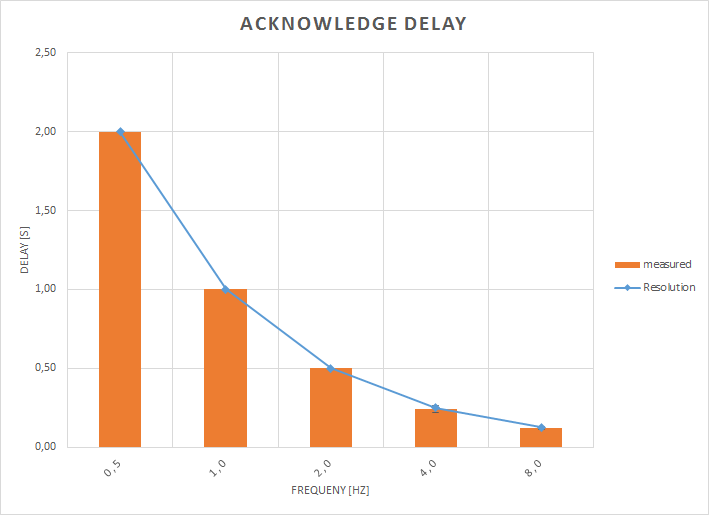
\includegraphics[scale=0.5]{content/images/exp3_norm.png}
		\caption{Acknowledge data rate (0.5Hz - 129Hz)}\label{fig:exp4norm}
	\end{figure}
	\begin{figure}[H]
		\centering
		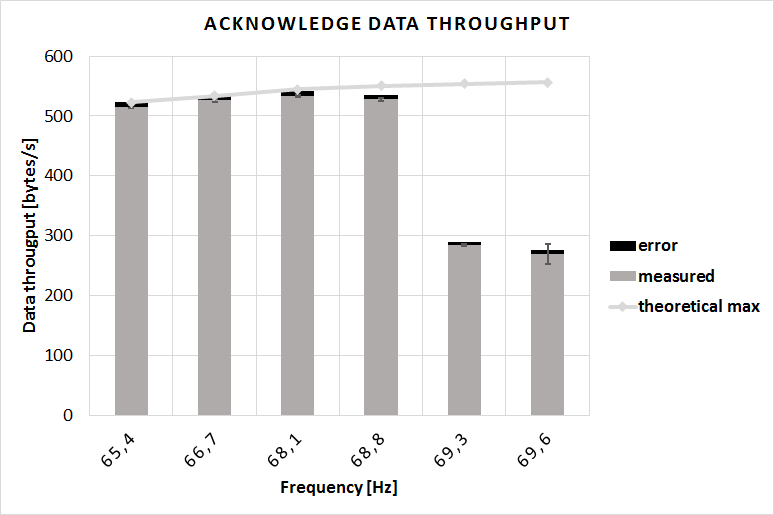
\includegraphics[scale=0.5]{content/images/exp3_detail.png}
		\caption{Acknowledge data rate (65Hz - 70Hz)}\label{fig:exp4between}
	\end{figure}
	
	Figure \ref{fig:exp4norm} shows the measured transmission speeds for the different tested frequencies. For the lower frequencies, the values align very well with the maximum data rate. Notable however is the drop off at 129 Hz. Figure \ref{fig:exp4between} shows the data throughput for some chosen values, between 64 Hz and 129 Hz. Demonstrating that the drop off starts around 69 Hz. 
	
	We conclude that the data throughput is a result of ANT retransmitting the last sent packet as broadcast data. If the frequency for this retransmission is too high it can interfere with the acknowledge message that the slave sends back to the master. For example at 128 Hz the message is broadcast every ~7 ms, resulting in too much data for the channel to handle. The transmission is thus interrupted. 
	Since there is no increase of the data throughput between 64 Hz and 128 Hz, but a huge drop off at 69 Hz it can be assumed that somewhere around 69 Hz the channel is at the maximum data throughput of around 1100 Bps. Again see section \ref{sec:dataThrougput} for a discussion about possible reasons for this upper limit. 	
\end{description}
\newpage

\section{Experiment 4: Acknowledge Transfer delay}
\begin{description} 
	\item{\textbf{Description}} \hfill \\ In this experiment we try to determine the time it takes for a node to receive and acknowledge a transmitted packet. The value is important in order to be able to determine the reaction time of SHAMPU to commands sent by the base station, for example to set up a separate channel for a burst transmission.
	\item{\textbf{Use-Case}} \hfill \\ Scheduled data-transmission
	\item{\textbf{Network topology and pseudo code}} \hfill \\ 
	\begin{figure}[H]
		\centering
		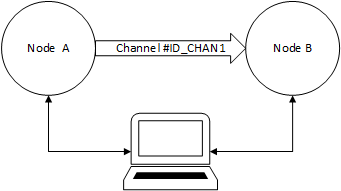
\includegraphics[scale=1]{content/images/exp_topo.png}
		\caption{Topology experiment 4}
	\end{figure}
	\begin{code}[H]
		\begin{verbatim}
		channelPeriod = max_Channel_Period
		while (channelPeriod >= min_Channel_Period) {
		  ANT_SetChannelPeriod(ID_CHAN1, channelPeriod);
		  ANT_OpenChannel(ID_CHAN1, ANT_Bidirectional_Master);
		  duration = 0.0
		  for (i in 0..10) {
		    ANT_SendAcknowledgedData(ID_CHAN1, [0x01, 0x02, 0x03, 0x04])
		    start = getTime()	   
		    wait_for_ack()		
		    print (getTime() - start) + " s"	  
		  ANT_CloseChannel(ID_CHAN1)		
		  if (channelPeriod >= 0x00FF)
		    channelPeriod = channelPeriod >> 1
		  else
		    channelPeriod = channelPeriod - 10
		\end{verbatim}
		\caption{Acknowledge data delay (Master)}\label{lst:mExp4}
	\end{code}
	
	\begin{code}[H]
		\begin{verbatim}
		channelPeriod = max_Channel_Period
		while (channelPeriod >= min_Channel_Period)
		  ANT_SetChannelPeriod(ID_CHAN1, channelPeriod);
		  ANT_OpenChannel(ID_CHAN1, ANT_Bidirectional_Slave);				 
		  wait_for_user_input();
		  ANT_CloseChannel(ID_CHAN1);
		  if (channelPeriod >= 0x00FF)
		    channelPeriod = channelPeriod >> 1
		  else
		    channelPeriod = channelPeriod - 10
		\end{verbatim}
		\caption{Acknowledge data delay (Slave)}\label{lst:sExp4}
	\end{code}
	
	\item{\textbf{Testing methodology}} \hfill \\ Node A acts as the master and node B as the slave. For both nodes the channel period is set to the highest value and the channel is opened. Node A then sends a total of 10 acknowledge messages and measures how long it takes until it receives the
	acknowledge signal. The channel period is then decreased and the experiment repeated.
	
	\newpage
	\item{\textbf{Result}} \hfill \\  
	\begin{figure}[H]
		\centering
		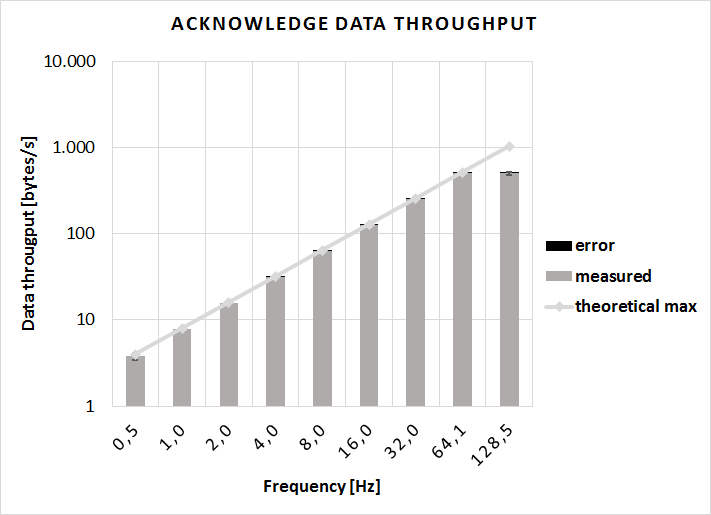
\includegraphics[scale=0.5]{content/images/exp4_norm.png}
		\caption{Acknowledge delay (0.5Hz - 8Hz)}\label{fig:exp3low}
	\end{figure}
	\begin{figure}[H]
		\centering
		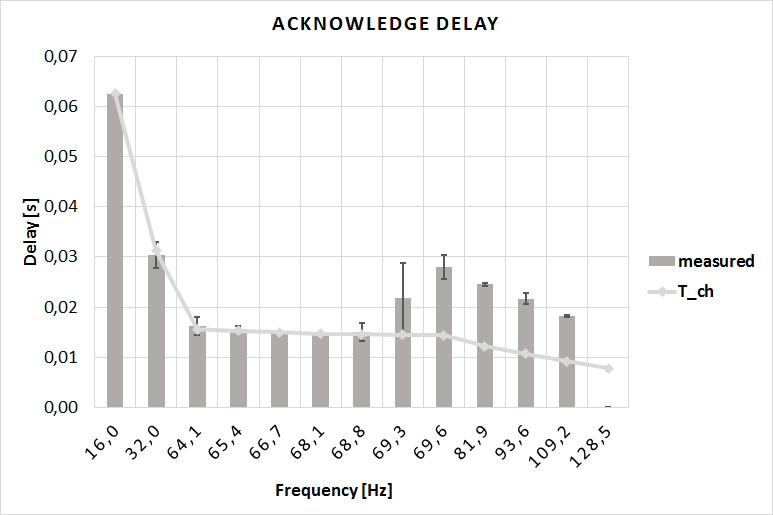
\includegraphics[scale=0.5]{content/images/exp4_detail.png}
		\caption{Acknowledge delay (16Hz - 70Hz)}\label{fig:exp3high}
	\end{figure}
	Figure \ref{fig:exp3low} and \ref{fig:exp3high} show the delays for the tested frequencies. The line shows the size of the gap between two timeslots and can act as a resolution for each measurement. For the lower frequencies the results are skewed, since each acknowledge packet is aligned to a time-slot. Thus, since ANT waits to send the acknowledge message the biggest part of the delay is waiting for the next time-slot. For frequencies greater than 64 Hz and below 68.8 Hz the data is considerably more useful, since the gap between two time-slots is lower than the measured values. The delay for those frequencies is around 18 ms, with no notable difference between 128 Hz and 200 Hz. Since the reply is always send directly after the message arrived, it can be assumed that the delay for the higher channel periods is the same as the one for the lower channel periods.
	
	The increase in the delay time for frequencies 68.8 Hz and greater can be explained with the results from experiment 3, where we determined that above 68 Hz the data throughput decreases. Since it is not possible to receive and send a package at the same time, the acknowledge message has to wait before it can be sent.
\end{description}
\newpage

\section{Experiment 5: Burst Data Transfer between two nodes}
\begin{description} 
	\item{\textbf{Description}} \hfill \\ Burst data transmissions make it possible to drastically increase the throughput rate. This allows a SHAMPU base station to quickly transmit a new firmware to a node or a node to dump its RAM back to the base station.	According to the  specification rates of up to 20 kbps can be achieved. To fully utilize this speed a baud rate of 50000 is needed. In the current set up the base station uses 19200 baud, since it is the only value that both the ANT chip and the RS-232 Interface support. Because of this we expect the maximum speed to be less than 20 kbps. Furthermore we try to determine whether the size of the burst transfer has an impact on the speed, since longer bursts will disrupt communications on other channels.
	\item{\textbf{Use-Case}} \hfill \\ Unscheduled data-transmission
	\item{\textbf{Network topology and pseudo code}} \hfill \\ 
	\begin{figure}[H]
		\centering
		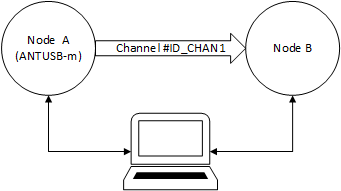
\includegraphics[scale=1]{content/images/exp5_topo.png}
		\caption{Topology experiment 5}
	\end{figure}
	\begin{code}[H]
		\begin{verbatim}
		size = START_SIZE
		ANT_OpenChannel(ID_CHAN1, ANT_Bidirectional_Slave);		
		while (size >= END_SIZE)
		  for (i in 0..10) 
		    // The first packet of a burst has the 3 MSB of the channelID field set to 0
		    wait_until(received_Packet == ANT_BURST_DATA && 
		               (received_message_channelID[0] & 0xE0) == 0x00)
		    start = getTime()
		    // The last packet of a burst has the MSB of the channelID field set to 1
		    wait_until(received_Packet == ANT_BURST_DATA && 
		               (received_message_channelID[0] & 0x80) > 0)		    
		  print (size - 1) / (getTime() - start) " Bytes per second"
		  size = 2 * size
		\end{verbatim}
		\caption{Burst data transfer (Slave)}\label{lst:sExp5}
	\end{code}
	\item{\textbf{Testing methodology}} \hfill \\ Since the burst transmission mode of our ANT-library is not working correctly (see section \ref{sec:future}) we use an ANTUSB-m Stick, which acts as a master. Node B is a normal base station and receives the burst transfers. On the master side, the program ANTWareII \cite{ANTwareII} is used to create the channel and then send bursts with different sizes. Each size is sent 10 times and the values are recorded and averaged. The size is then doubled and the experiment repeated. The first burst packet cannot be counted directly since the start of the burst can only be determined after the ANT chip has already received the first packet.
	\newpage
	\item{\textbf{Result}} \hfill \\ 
	\begin{figure}[H]
		\centering
		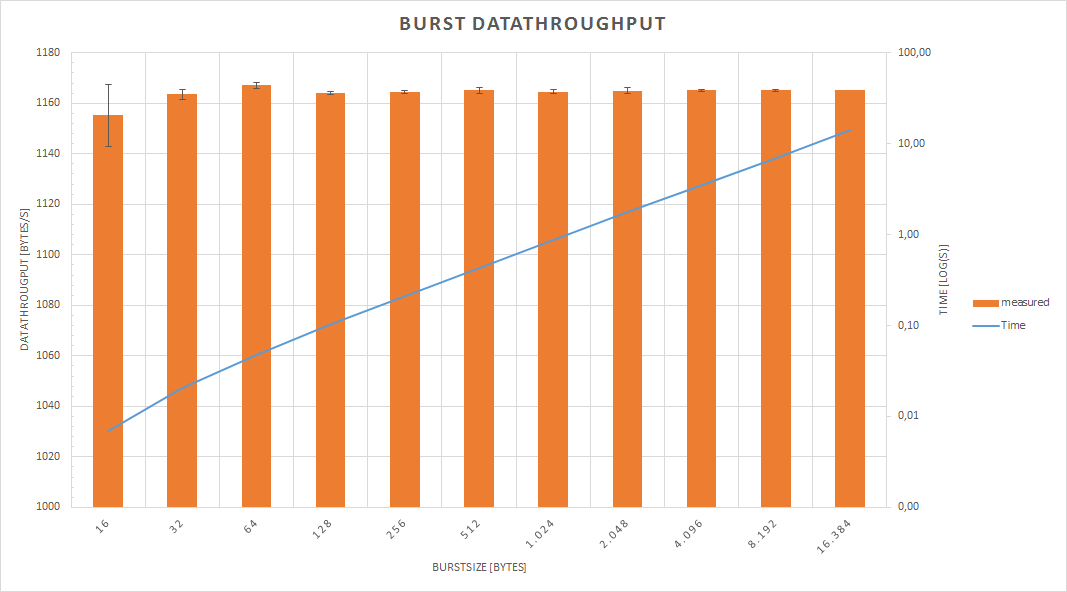
\includegraphics[scale=0.5]{content/images/exp5.png}
		\caption{Burst data rate}\label{fig:exp5}
	\end{figure}
	Figure \ref{fig:exp5} shows the achieved data rates for the different packet sizes and also the length of the transfer. As seen the values all hover around the same value of ~1165 Bps. This is approximately the same value as the one which can be achieved with the other two types of data.
	Again see section \ref{sec:dataThrougput} for a discussion about possible reasons for this upper limit. 
\end{description}
\newpage

\section{Experiment 6: Maximum communication Range}
\begin{description} 
	\item{\textbf{Description}} \hfill \\  In this experiment we try to determine the correlation between the maximum range and the power setting of the ANT radio. One of SHAMPU's advantages is the low power consumption, so it might be possible to further reduce the power consumption by decreasing the power level of the ANT radio, especially in smaller environments where there is no need for such a range. According to the datasheet the maximum range for communication is 30m, however the ANT documentation does not provide different ranges for different power settings. 
	
	\item{\textbf{Use-Case}} \hfill \\ Unscheduled data-transmission and scheduled data-transmission	
	\item{\textbf{Network topology and pseudo code}} \hfill \\ 
	\begin{figure}[H]
		\centering
		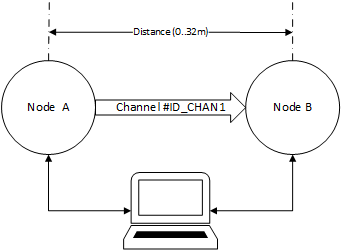
\includegraphics[scale=1]{content/images/exp6_topo.png}
		\caption{Topology experiment 6}
	\end{figure}
	
	\begin{code}[H]
		\begin{verbatim}
		for (pSetting in Available_PowerSettings)
		  ANT_SetTransmitPower(pSetting)
		  openChannel(ID_CHAN1, ANT_Bidirectional_Master)
		  ANT_SendBroadcastData(ID_CHAN1, [0x01, 0x02, 0x03, 0x04])
		  wait_for_user_input();
		  closeChannel(ID_CHAN1);
		\end{verbatim}
		\caption{Maximum communication range (Master)}\label{lst:mExp6}
	\end{code}
	
	\begin{code}[H]
		\begin{verbatim}
		distance = 0.0
		stopInc = false
		loop 
		  openChannel(ID_CHAN1, ANT_Bidirectional_Slave)
		  wait_until(received_Packet == ANT_BROADCAST_DATA || 
		             received_Packet == ANT_MESSAGE_EVENT_RX_SEARCH_TIMEOUT) 
		  if (stopInc) 
		    if (wasTimeout) 
		      distance -= .4
		    else 
		      print "Connection found : " + distance
		  else
		    if (wasTimeout)  
		      stopInc = true
		      distance -= .4
		      print "Connections lost : " + distance
		    else distance += .4
		  closeChannel(ID_CHAN1);
		\end{verbatim}
		\caption{Maximum communication range (Slave)}\label{lst:sExp6}
	\end{code}
	\item{\textbf{Testing methodology}} \hfill \\ At the beginning of the experiment Node A and B are placed right next to each other. Node A acts as a master and keeps broadcasting the same message. Node B is the slave and tries to connect to the channel. If the connection is successful, the distance between the two nodes is increased by 0.4 meters. This process is repeated until Node B can no longer connect to the channel and the connection times out. This happens after 30s of searching. At this point the distance is no longer increased, but rather decreased until Node B is able to successfully connect to the channel. Both of these values are recorded. The whole experiment is then repeated for each available power setting.	
	\newpage
	\item{\textbf{Result}} \hfill \\ 
	\begin{figure}[H]
		\centering
		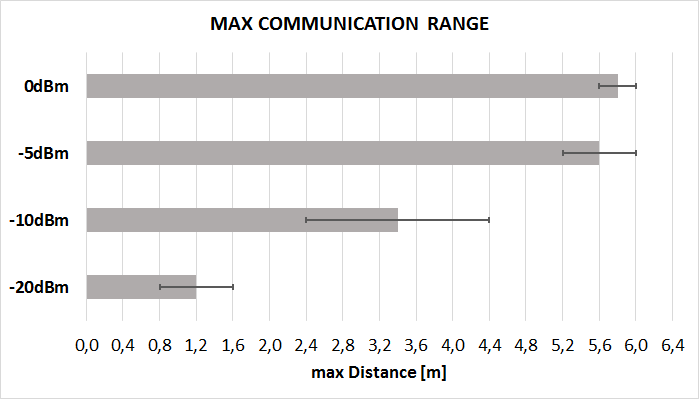
\includegraphics[scale=0.5]{content/images/exp6.png}
		\caption{Maximum comunication range}\label{fig:exp6}
	\end{figure}
	Figure \ref{fig:exp6} shows the transmission range for each power setting. As expected the maximum distance goes up with the higher power settings. But the result at the highest power setting is disappointing, since we did not get close to the claimed maximum range of 30m. The ANT documentation states that the maximum range of 30m can only be achieved in "optimal conditions" \cite{DynastreamInnovationsInc.2013}. It is possible for several different unfavorable factors to interfere with the ANT signal, such as multiple 802.11 networks in the vicinity, or even the plastic case of the base station. 
\end{description}

\newpage
\section{Maximum Data Throughput}
\label{sec:dataThrougput}

In our experiments we were able to confirm two important limits for the maximum data throughput which can be achieved with our current set up. The ANT AP1MxIB supports a maximum message frequency of 200 Hz, which means that we would expect to see a maximum transmission rate of 1600 Bps.
However, this limit can only be achieved by splitting the available bandwidth between receiving and sending. If we try to utilize the full 200 Hz only for either receiving or sending, we are limited to 1100 Bps, around 500 Bps or 30\% lower than the theoretical maximum. The same 1100 Bps limit holds for burst transmissions, where we loose around 1100 Bps or 56\% of the maximum data throughput.\\

To balance environmental influences, the experiments were repeated in different locations and times of day and night. Since the throughput did not change noticeably, it can be assumed that there are no easily eliminated environmental factors affecting the maximum rate. We conclude that the root cause for the lower than expected throughput must be attributed to the hardware or software. \\

If we exclude environmental factors, the limitations could be based on certain parts of the test set up:
\begin{itemize}
	\item{\textbf{RS-232 Connection}} \hfill \\ The base station is connected to a PC over a serial connection. For the speed we chose 19200 baud, since it is the highest value supported by the ANT chip and the serial-Interface. With 19200 baud the maximum data rate of the RS-232 Connection is 1920 Bps, since the interface adds a start and stop bit to each byte. This data rate is enough for the maximum message frequency. If the serial connection would be the bottle neck for burst transmission, we would expect to get the full 1920 Bps of data throughput. Since this is not the case we can conclude that the RS-232 connection is not the limiting factor. This is supported by the same limits for broadcast and burst transmissions.

	\item{\textbf{ANT API}} \hfill \\ The software we use is not officially supported by ANT. It is thus possible that there are some bugs which have an impact on the performance. Except for the missing burst mode (see \ref{sec:future}), there were no unusual measured values during the experiments. If there is a bug, it might be hard to find without rewriting all the experiments and running them with the official ANT library \cite{ANTWinLib}
	
	\item{\textbf{ANT AP1MxIB}} \hfill \\ Due to the black box nature of ANT, it is very hard to exactly determine what causes the problem. The inner workings of the chip are not documented in any way, and the error messages of the protocol are not very specific. We suspect that the ANT chip receiver and sender are somehow limiting the maximum data throughput. The chip itself is from 2007 and the manufacturer no longer recommends the use of the chip\cite{AP1page}. There are alternatives available, like the newer ANTAP281M5IB chip \cite{AP2Datasheet}.
\end{itemize}
\newpage